% Document class options:
% 11pt for 11 point font
% oneside for not weird margins between odd and even pages
% (omitting oneside gives a better margin setup for print
% but i'm guessing  you're handing this in)
% a4paper to A4 page size, because LaTeX by default is setup
% to use US Letter paper size, because Donald Knuth
% the article class, as the book class is designed for
% larger documents and you probably don't need chapter
% environments
\documentclass[11pt, oneside, a4paper]{article}
\usepackage[utf8]{inputenc}
\usepackage[english]{babel}

\usepackage{hyperref}
\hypersetup{
    colorlinks=true,
    linkcolor=blue,
    filecolor=magenta,      
    urlcolor=cyan,
}

\urlstyle{same}
% Set spacing (i set it to 1.2x)
\renewcommand{\baselinestretch}{1}
% Indentation (set this to zero for normal prose)
\setlength{\parindent}{0em}
% Line breaking (spacing between paragraphs)
\setlength{\parskip}{0.5em}

% Use the whole page
\usepackage{geometry}
% Extra math glyphs
\usepackage{amsmath}
% Proper enumerate spacing
\usepackage{enumitem}
% More pleasing screen fonts
\usepackage{lmodern}
% Fancy headers
\usepackage{fancyhdr}
\usepackage{graphicx}
% Allows absolute positioning of images
\usepackage{float}

% Set no separation
\setlist{noitemsep}
% Set margins to reasonable
\geometry{margin=2.5cm}
% Sets graphics path
\graphicspath{ {./images/} }
% Sets up fancy headers
\pagestyle{fancy}
\fancyhf{}
\lhead{Natalie Hong Visualization Project Proposal}
\rhead{COSC3000}

\begin{document}
\section*{Introduction}
Hi, my name is Natalie Hong and I am a third year Software Engineering Student. I have chosen to take this course as I enjoy visualising data and am super interested in the graphics section of the course as I was able to brush over it in highschool, but was never able to further my knowledge in it.
I also am heavily involved in a certain gaming community which has serves as the main factor of choice for my visualization project decision.

\section*{What?}
What I will be visualising will be Australian character data usage, skill gain and matches played throughout 2019 for the game Super Smash Bros. Ultimate for the Nintendo Switch. 
Since I am using an API and the data is always updating, I will be sorting each set of data into states and then into individual quarters of 2019 so that data is static rather than a dynamic approach.
Data is stored as a JSON and CSV files and will be visualised on a webpage as I would like it to be publically viewed when the project is completed as well as being interactive to an extent.

With six points of data to use (state, character name, players, elo gain/skill ranking per character, matches played, quarter), a comparrison for each state per quarter can be graphed as well as the possiblity 3-axis graphs. It will also be possible to compare the whole of Australia by quarters due to this multivariate data set.

Possible graphs that could be used to display different data sets that I see fitting for my project could and are not limited to:
\begin{itemize}
    \item Bubble graphs
    \item Bar graphs
    \item Line graphs
    \item Heat maps
    \item 3D plots in matlab
    \item Scatterplots
\end{itemize}

\section*{Why?}
The reason that I want to undertake this project is to answer various questions about character data within Australia. These questions that I want to be able to answer at the end of this project are as follows:
\begin{itemize}
    \item Does the amount of players influence the elo gain?
    \item Do more players mean better results?
    \item Which state has the best performing characters?
    \item Who are the top 5 most played characters in each state?
    \item What is the relation between top played characters and elo distribution?
    \item Which state has the most unique character usage compared to other states?
    \item How did the 'meta' of charcter usage change between each quarter?
\end{itemize}
When mentioning character usage, a select top few characters (5 - 10) will be taken from the total list will be used rather than the 70+ characters in the game to allow for better viewing and less confusion. It will also allow me to be able to see how each graph changes over time.

\section*{How?}
To achieve the visualization page that I want I will use the following tools:
\begin{itemize}
    \item Python 3 to run API calls
    \item Google charts and Matlab for graphing
    \item Ausmash API \href{https://api.ausmash.com.au/swagger/ui/index#/}{(Click for Documentation)}
    \item JQuery for Interaction display
    \item JSON and CSV files to store and display data
\end{itemize}

\section*{Example Visualization}
Before beginning the data collection and shuffling, I decided to make some very basic designs for what the final visualisations could look like. These designs were as follows:

\subsection*{Bubble Graph}
{%
\setlength{\fboxsep}{0pt}%
\setlength{\fboxrule}{1pt}%
\fbox{
    \includegraphics[scale=0.25]{BubbleChart.png}%
}%

Bubble graphs were the original source of inspiration for this project. Shows the amount of unique people who play the character (radius) vs elo gain (x-axis) and the number of matches played (y-axis).

\subsection*{Bar Graphs}
{%
\setlength{\fboxsep}{0pt}%
\setlength{\fboxrule}{1pt}%
\fbox{
    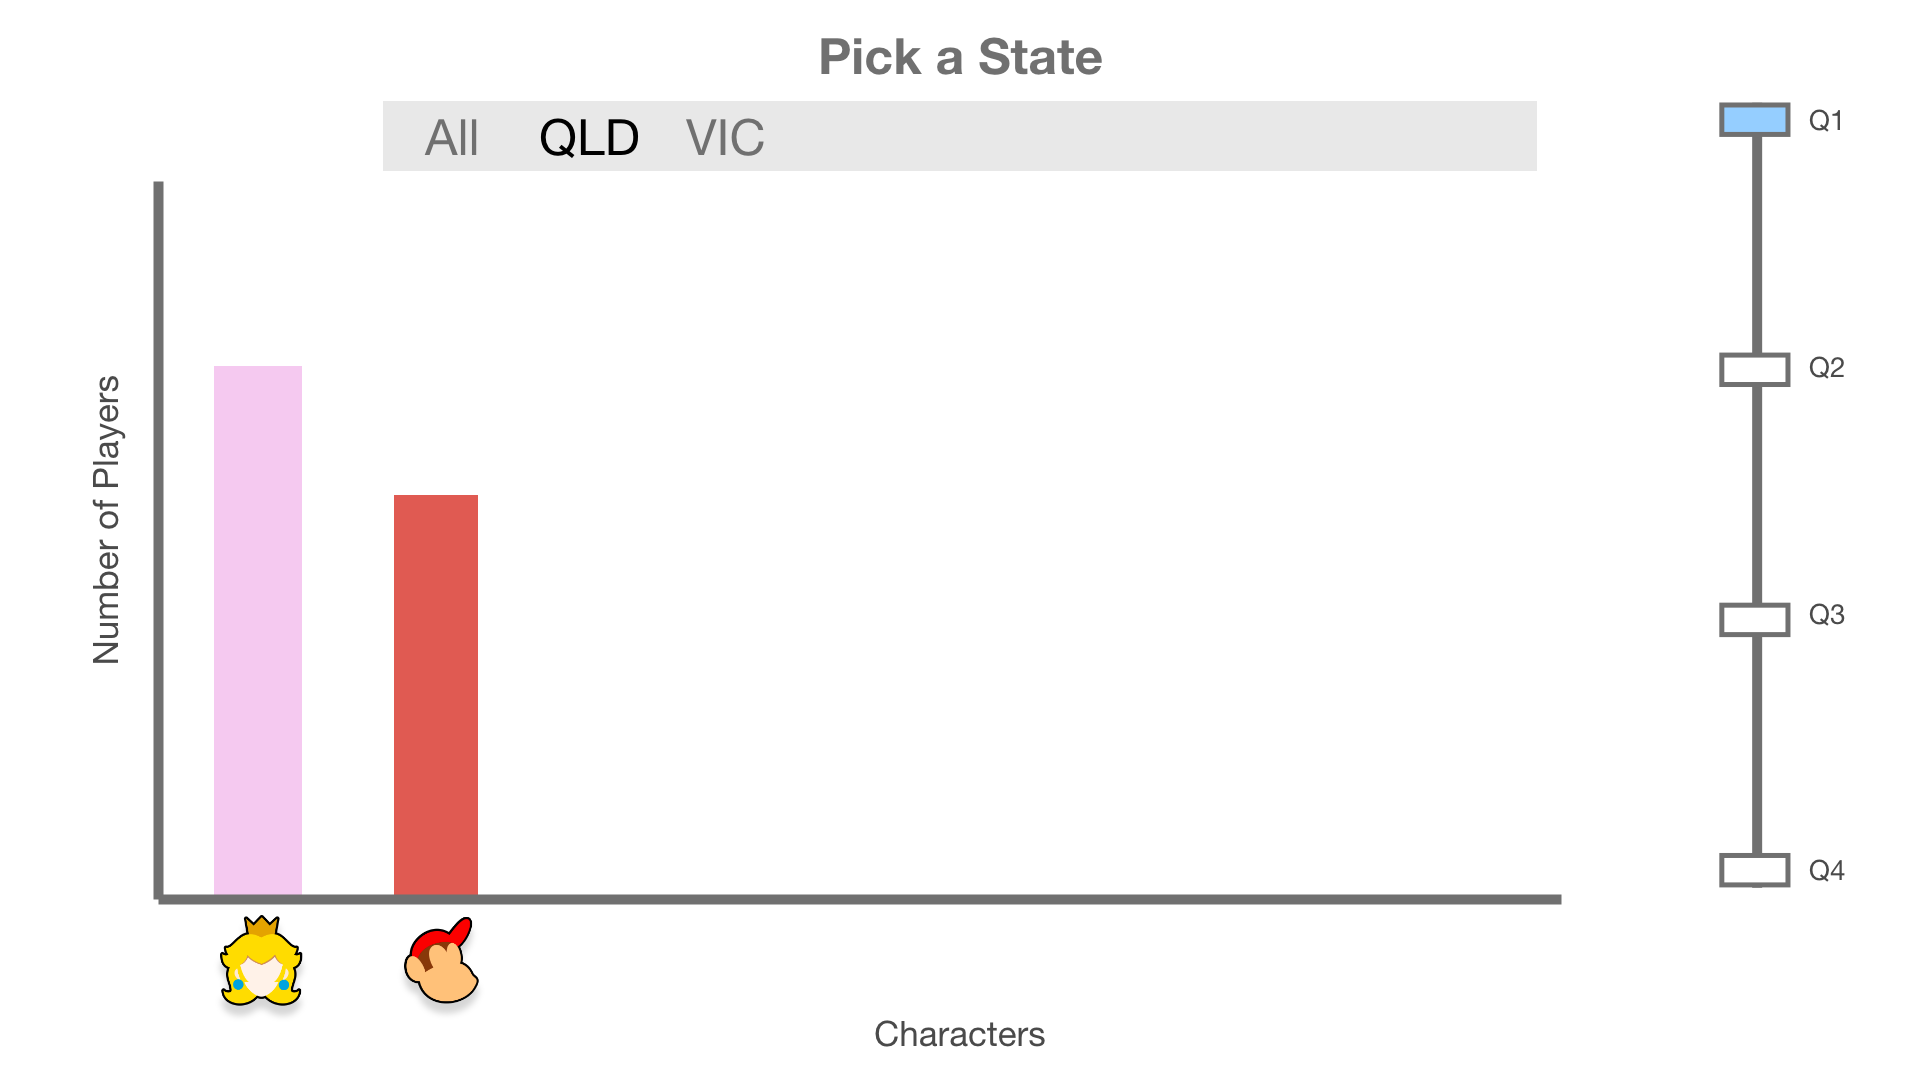
\includegraphics[scale=0.25]{BarChart1.png}%
}%

Bar chart 1 which shows the amount of unique individuals who play each character in each state in each quarter.

{%
\setlength{\fboxsep}{0pt}%
\setlength{\fboxrule}{1pt}%
\fbox{
    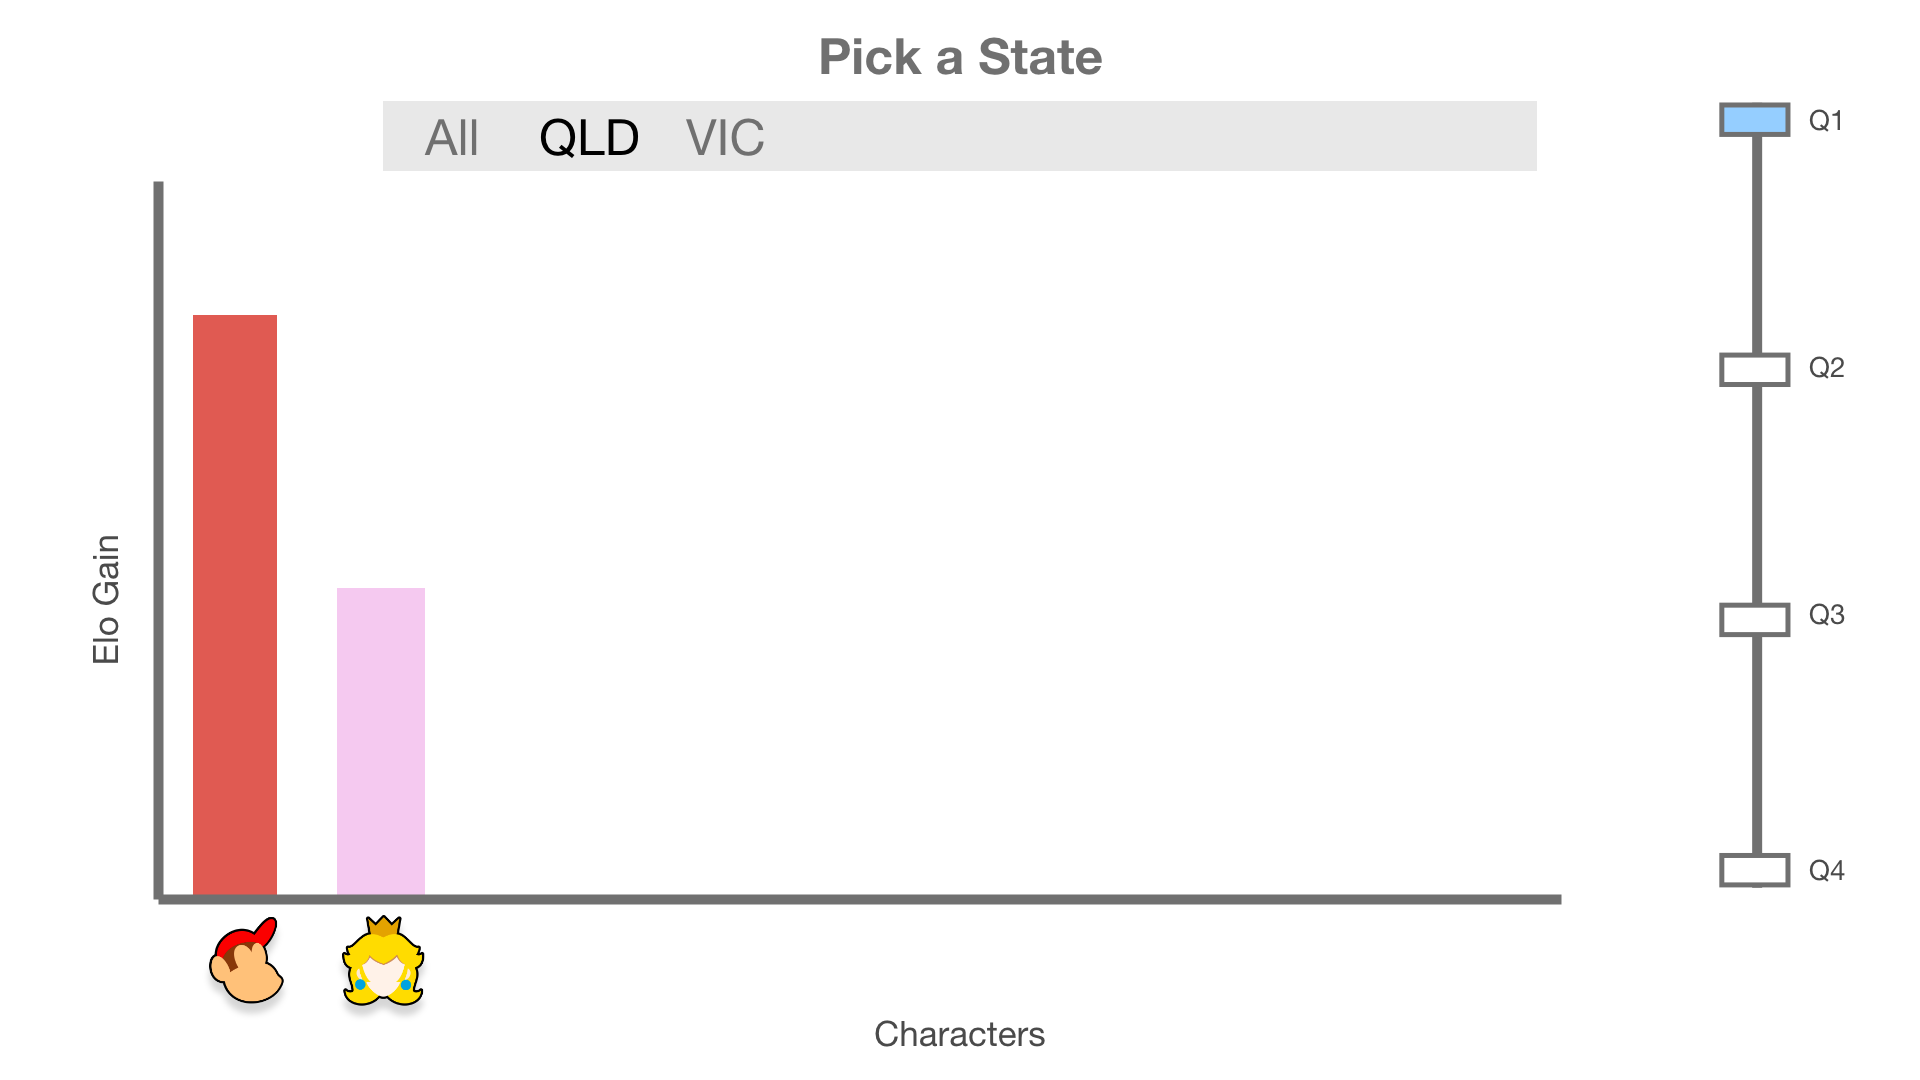
\includegraphics[scale=0.25]{BarChart2.png}%
}%

Similar to bar chart 1 but instead of individuals, it shows elo gain per quarter per state.

\subsection*{Line Graphs}

{%
\setlength{\fboxsep}{0pt}%
\setlength{\fboxrule}{1pt}%
\fbox{
    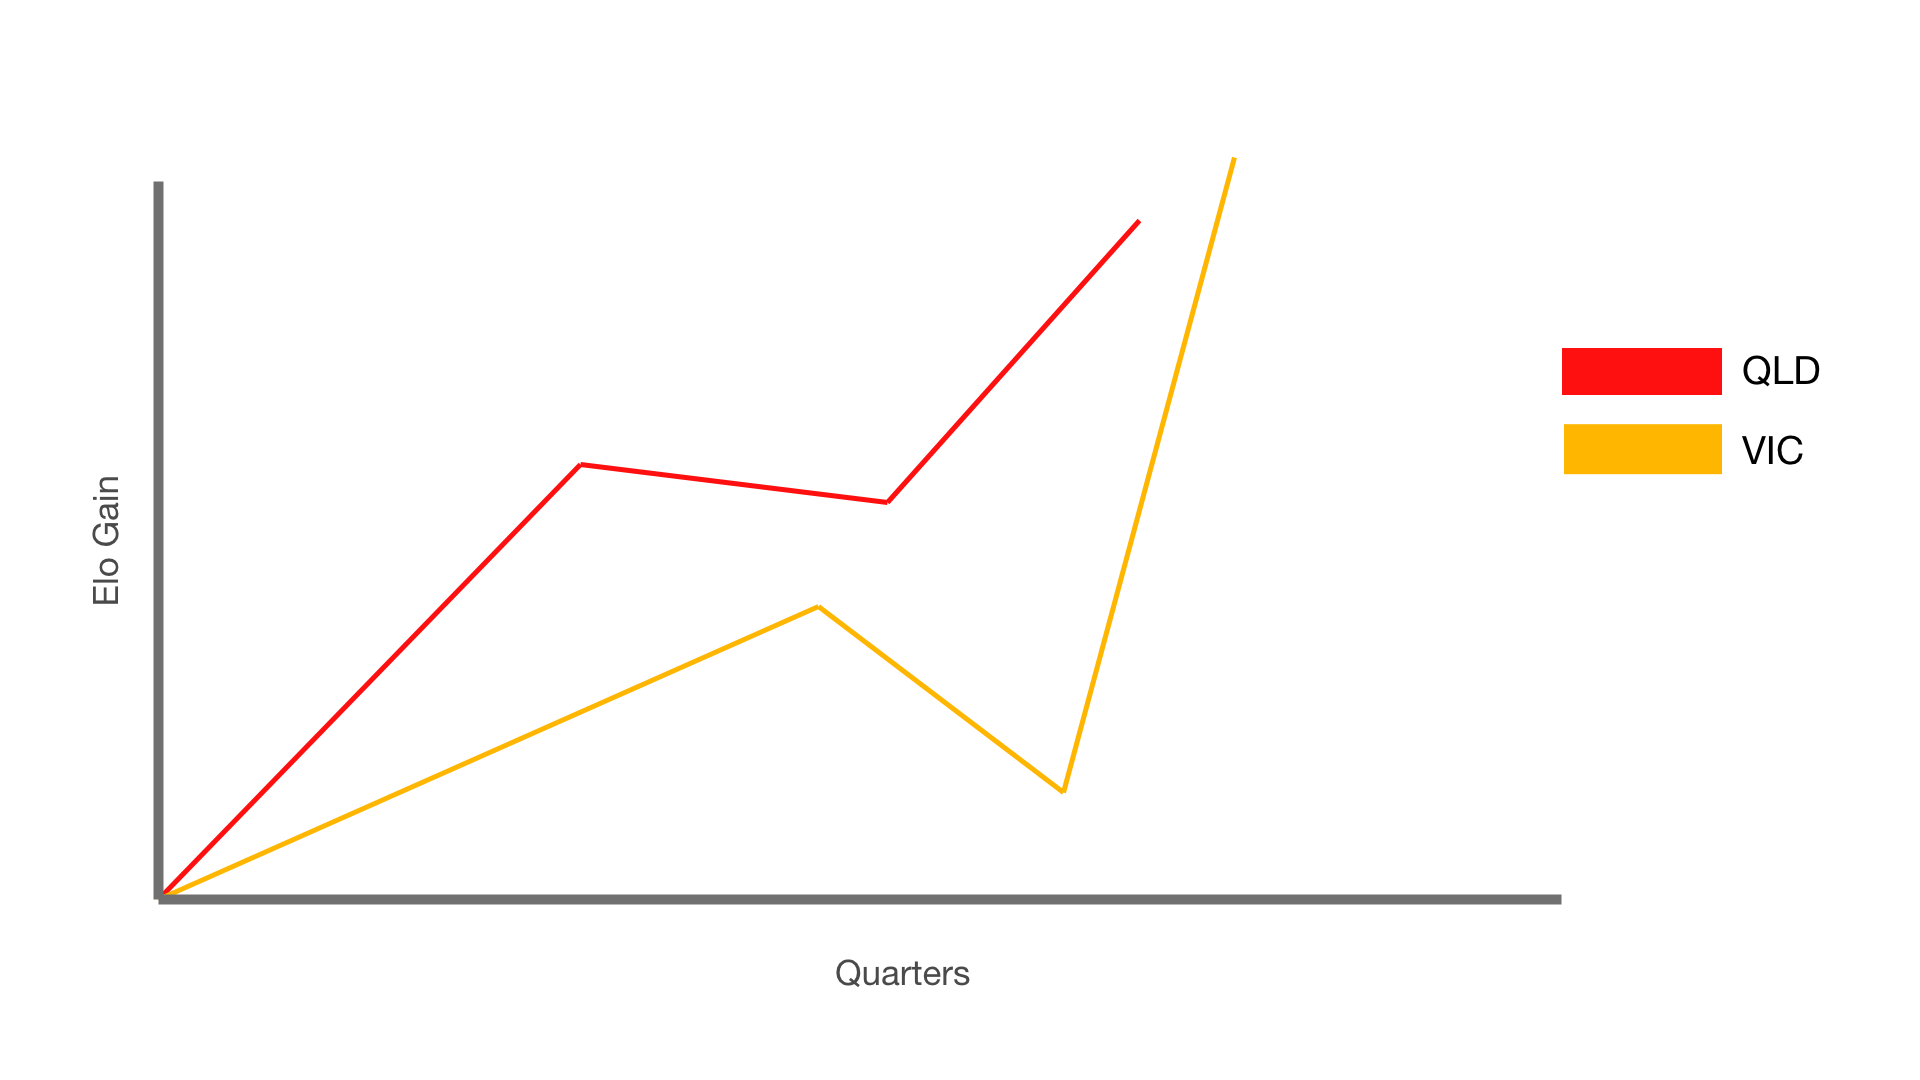
\includegraphics[scale=0.25]{LineGraph1.png}%
}%

Line Graph 1 could graph the amount of elo gain for each state over each quarter of the 2019 season.

{%
\setlength{\fboxsep}{0pt}%
\setlength{\fboxrule}{1pt}%
\fbox{
    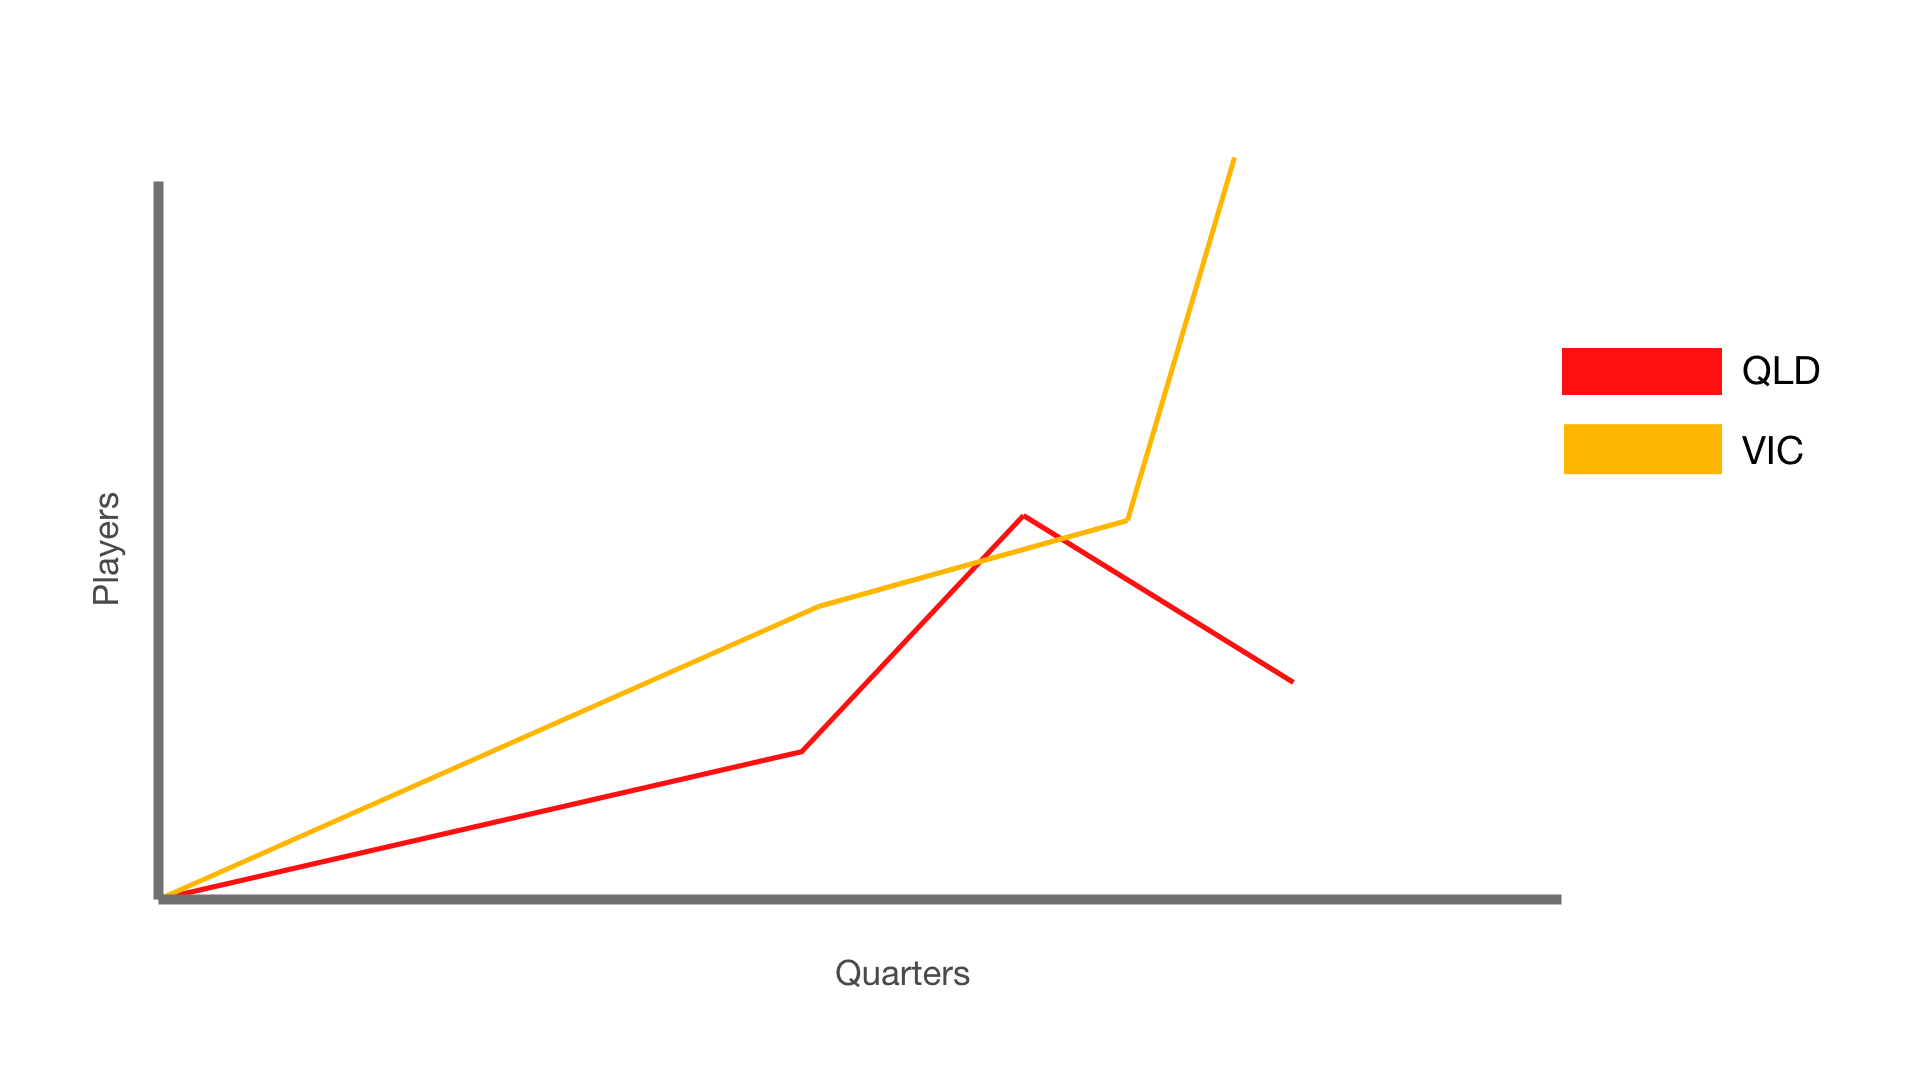
\includegraphics[scale=0.25]{LineGraph2.png}%
}%

Line Graph 2 is similar to the first graph except instead of elo, the number of players is used. 

\section*{Conclusion}
Overall, I hope you are enlightened to my visualisation idea and the data I have chosen to use, sorry it was so long. I am really looking forward to implementing this (and hopefully passing this proposal).
- Nat

\end{document}